\chapter{Oscillation Probability Calculation}
\label{chap:OscillationProbability}

\section{Overview}
\label{sec:Oscillation_Overview}

The analysis presented within this thesis focuses on the determination of oscillation parameters from atmospheric and beam neutrinos. Whilst subject to the same oscillation probability, the way in which the two sets of samples have sensitivity to the different oscillation parameters differs quite significantly.

Atmospheric neutrinos have a varying baseline, or ``path length'', such that the distance each neutrino travels before interacting is dependent upon the zenith angle. Therefore the oscillation probability can be represented as a two-dimensional ``oscillogram'' as shown in \autoref{fig:Oscillation_SK_BasicOscillogram}. For this calculation, four layers of fixed density were used to model the Earth with values taken from an approximation of the PREM model. These can be seen in the distinct discontinuities in the oscillogram as a function of the zenith angle.

Another complexity of atmospheric neutrino oscillation probability calculation is the uncertainty in the height at which a neutrino was produced, termed the ``production height''. Primary cosmic rays, whch contribute most of the neutrino flux, can interact anywhere between the Earth's surface and \quickmath{\sim50\text{km}} above that. The baseline, \quickmath{L}, for a neutrino generated with zenith angle, \quickmath{\theta}, and production height, \quickmath{h}, can be calculated as

\begin{equation}
  L = \sqrt{\left(R_{E} + h\right)^{2} - R_{E}^{2} \left(1 - \cos^{2} \left(\theta \right) \right)} - R_{E}\cos(\theta),
\end{equation}

where \quickmath{R_{E} = 6,371\text{km}} is the Earth's radius.

\begin{figure}[h]
  \begin{subfigure}[t]{0.8\textwidth}
    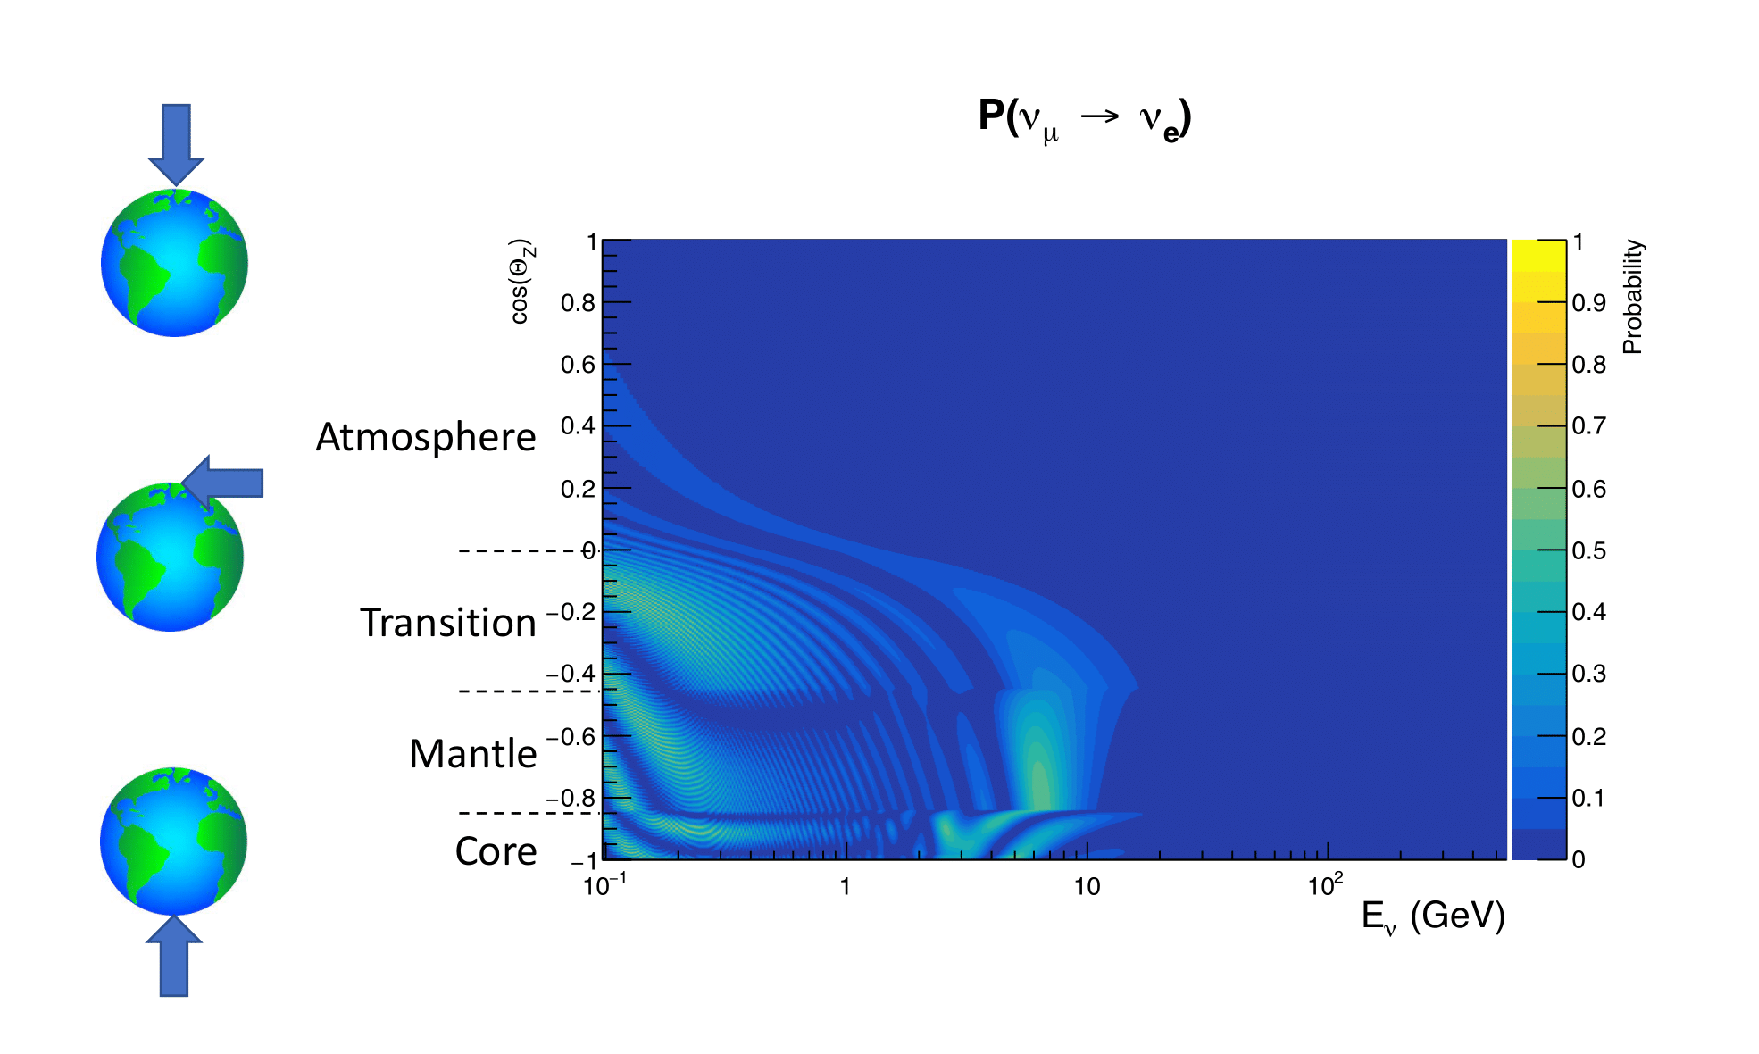
\includegraphics[width=\textwidth, trim={0mm 0mm 0mm 0mm}, clip,page=1]{Figures/Oscillation/BasicOscillogramWithNotes.pdf}
  \end{subfigure}
  \caption{An ``Oscillogram'' that depicts the \quickmath{P(\nu_\mu \rightarrow \nu_e)} oscillation probability as a function of neutrino energy and cosine of the zenith angle. The zenith angle is defined such that \quickmath{\cos(\theta_{Z}) = 1.0} represents neutrinos that travel from directly above the detector. The four-layer constant density PREM model approximation is used and Asimov A oscillation parameters are assumed.}
  \label{fig:Oscillation_SK_BasicOscillogram}
\end{figure}

Atmospheric neutrinos do have some sensitivity to \dcp through a normalisation term. \autoref{fig:Oscillation_SK_DCPSensitivity} illustrates the difference in oscillation probability between CP-conserving and CP-violating \dcp values. The result is a complicated oscillation pattern in the appearance probability for sub-GeV upgoing neutrinos. The detector does not have sufficient resolution to resolve these individual patterns so the sensitivity to \dcp for atmospheric neutrinos comes via the overall normalisation of the sub-GeV upgoing events. The presence of matter means that the effect \dcp has on the oscillation probability is not equal between neutrinos and antineutrinos which would be expected when propagating through a vacuum. This is further extenuated by the fact that SK can not distinguish neutrinos and antineutrinos well and that the cross-section neutrino interaction is larger than that for antineutrinos. Finally, sample selections (discussed in \finish{Link to selection chapter}) targeting different neutrino interaction modes (charge current quasi-elastic and single pion production) result in an imbalance in the percentage of neutrinos to anti-neutrinos in these samples due to pion capture. Negatively charged pions from antineutrino interactions are more likely to be captured by a nucleus compared to a positively charged pion emitted from a neutrino interaction. This all culminates in atmospheric neutrinos having a very complex sensitivity to \dcp.

\begin{figure}[h]
  \begin{subfigure}[t]{\textwidth}
    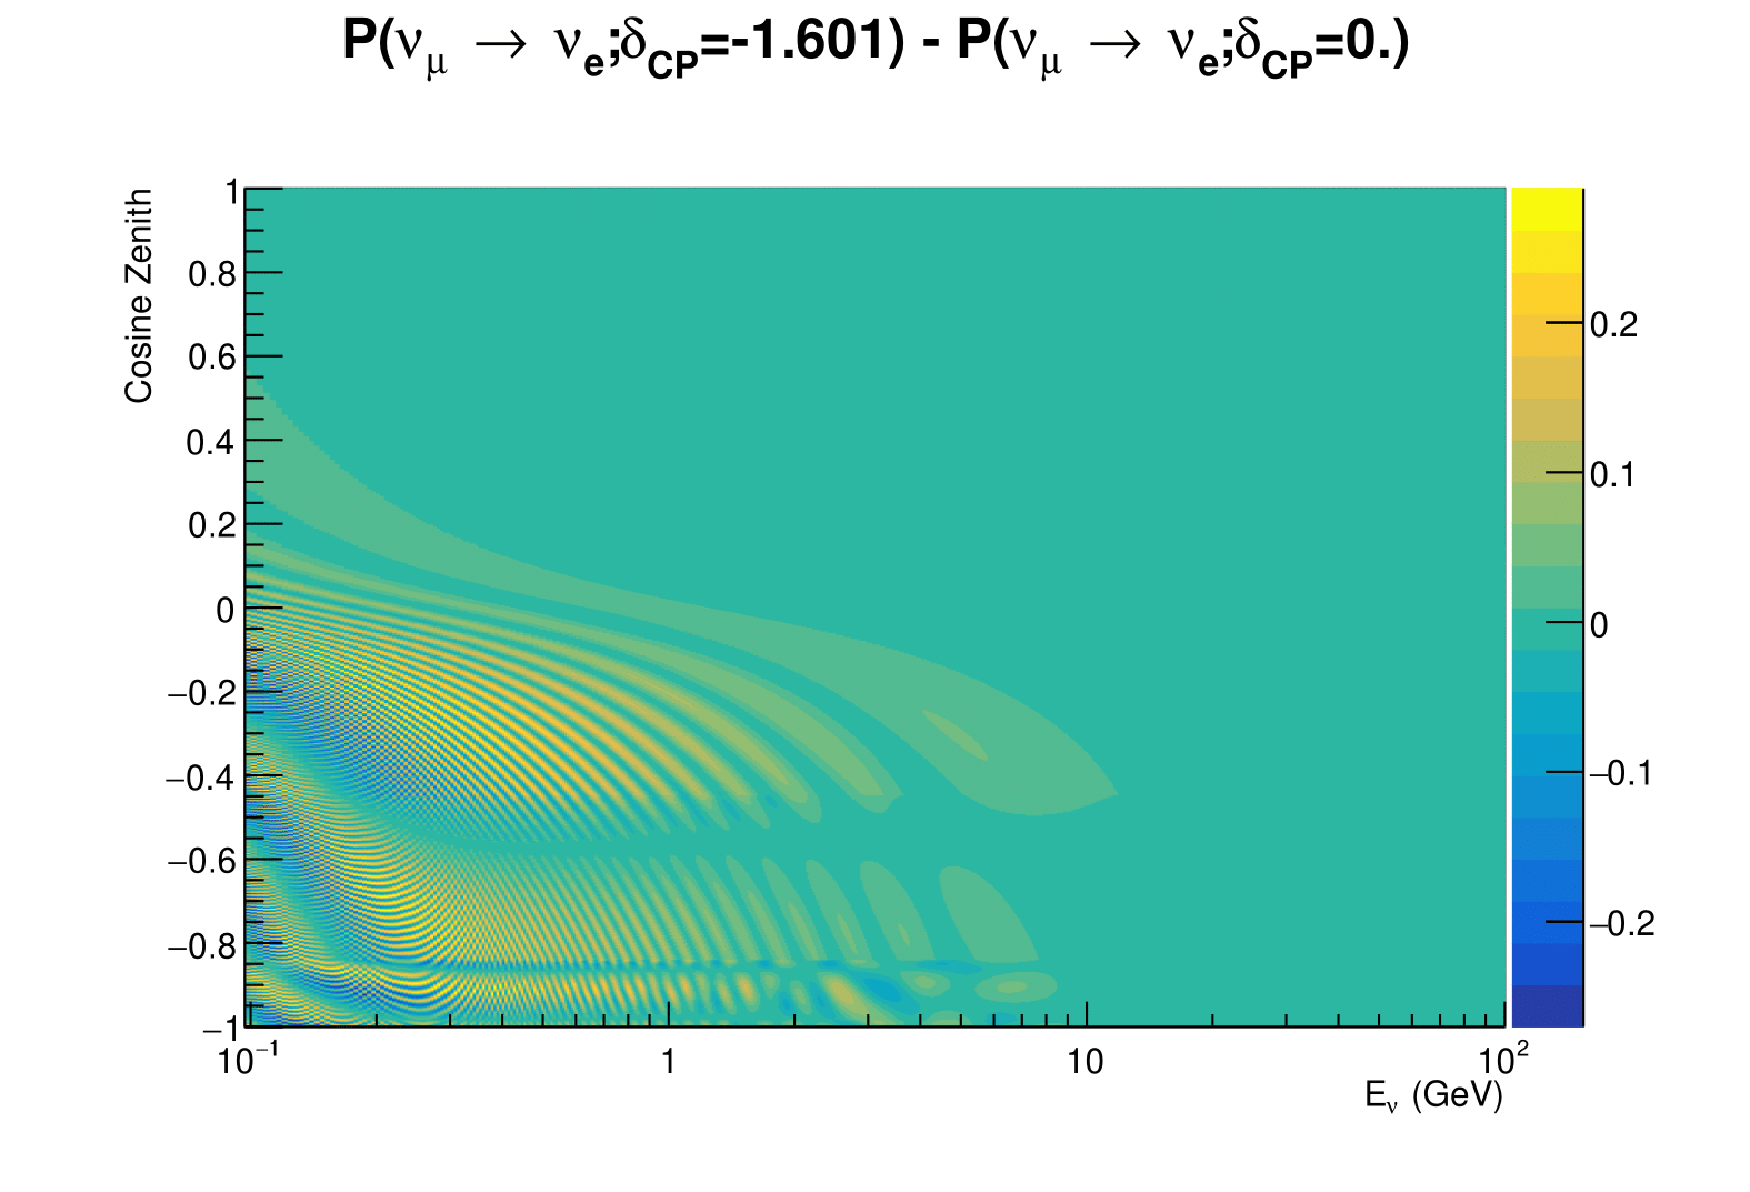
\includegraphics[width=\textwidth, trim={0mm 0mm 0mm 0mm}, clip,page=1]{Figures/Oscillation/AtmDCPSens.pdf}
  \end{subfigure}
  \caption{The effect of \dcp for atmospheric neutrinos given in terms of the neutrino energy and zenith angle. The oscillogram compares the \quickmath{P(\nu_{\mu} \rightarrow \nu_{e})} oscillation probability for a CP conserving (\quickmath{\delta_{CP}=0.0}) and CP violating (\quickmath{\delta_{CP}=-1.601}) value of \dcp. The other oscillation parameters assume the ``Asimov A'' oscillation parameter set given in \autoref{tab:Oscillation_ParameterSets}.}
  \label{fig:Oscillation_SK_DCPSensitivity}
\end{figure}

Atmospheric neutrinos are subject to matter effects as they travel through the dense matter in the Earth. The vacuum and matter oscillation probabilities for \quickmath{P(\nu_{e} \rightarrow \nu_{e})} and \quickmath{P(\bar{\nu}_{e} \rightarrow \bar{\nu}_{e})} are presented in \autoref{fig:Oscillation_SK_VacuumMatter}. The oscillation probability for both neutrinos and antineutrinos are affected in the presence of matter but the resonance (Effects around \quickmath{E_{\nu} \sim 5\text{GeV}}) only occurs for neutrinos in normal mass hierarchy and antineutrinos for inverse mass ordering. The exact position and amplitude of the resonance depend on \sinsqatm meaning that the atmospheric neutrinos have sensitivity to the octant of \quickmath{\theta_{23}}. 

\begin{figure}[h]
  \begin{subfigure}[t]{\textwidth}
    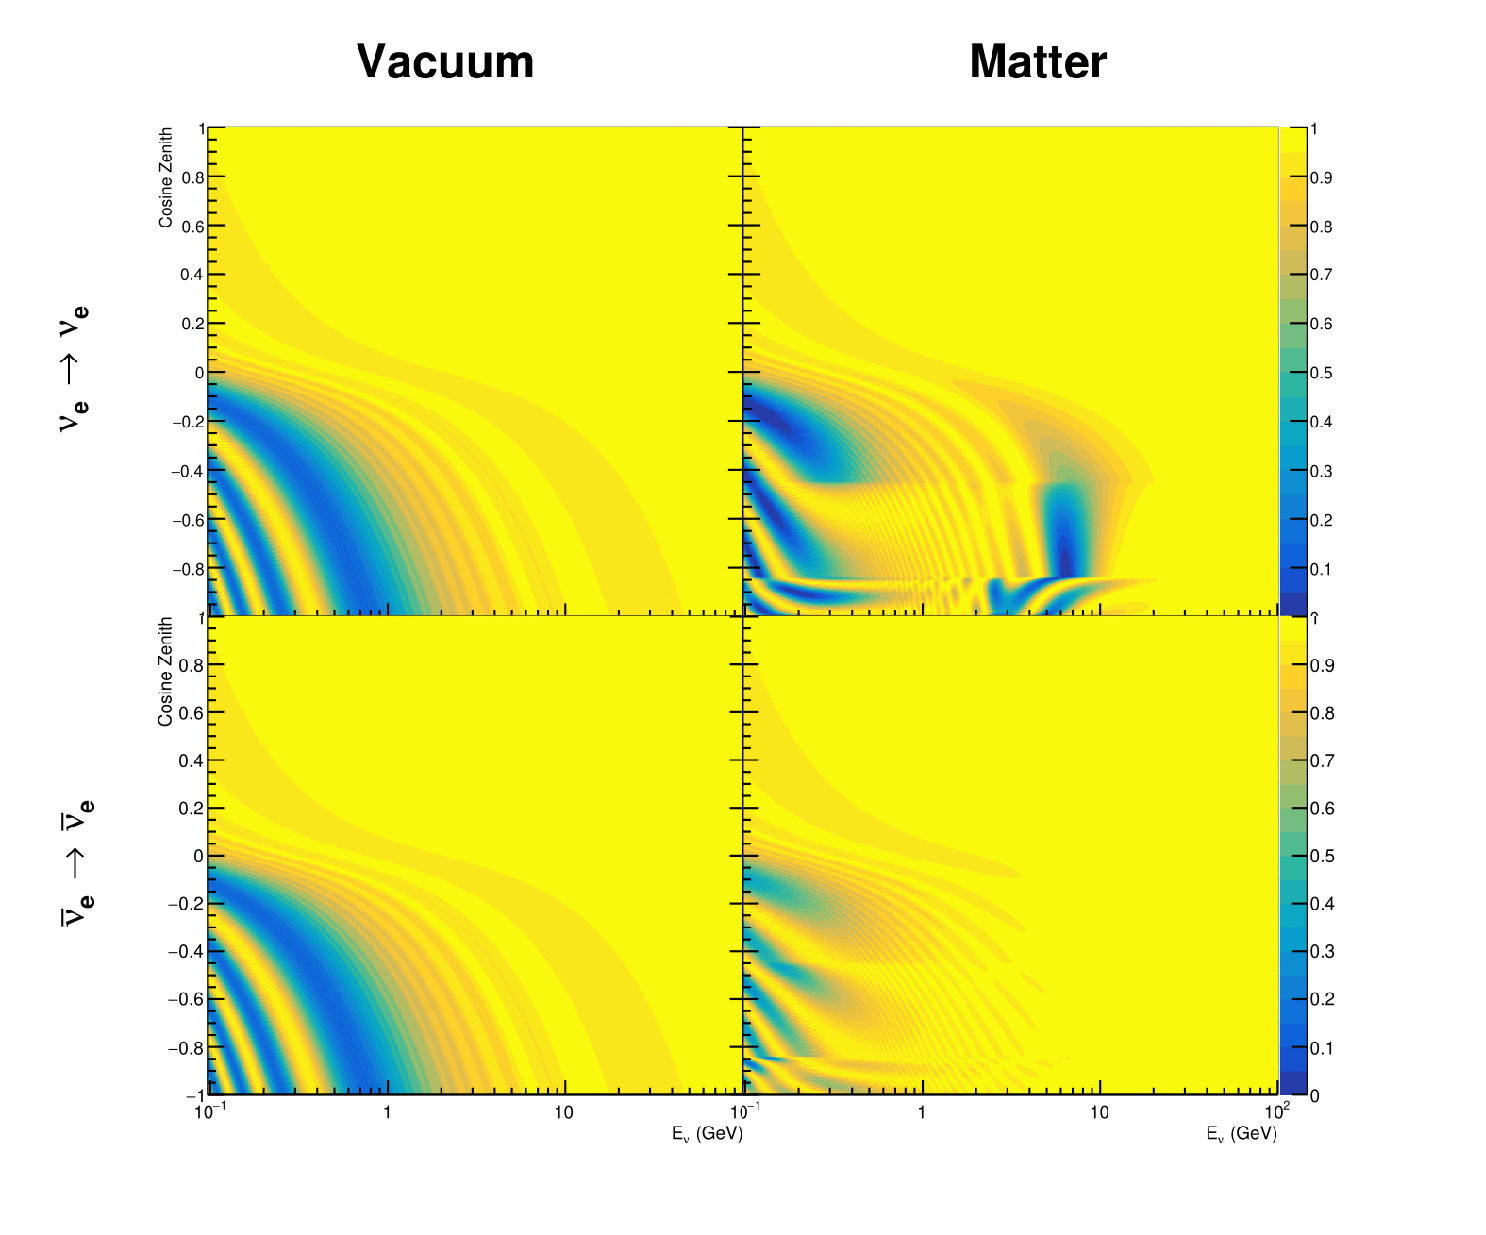
\includegraphics[width=\textwidth, trim={0mm 0mm 0mm 0mm}, clip,page=1]{Figures/Oscillation/MatterEffect.pdf}
  \end{subfigure}
  \caption{An illustration of the matter-induced effects on the oscillation probability, given as a function of neutrino energy and zenith angle. The top row of panels gives the \quickmath{P(\nu_{e} \rightarrow \nu_{e})} oscillation probability and the bottom row illustrates the \quickmath{P(\bar{\nu}_{e} \rightarrow \bar{\nu}_{e})} oscillation probability. The left coloumn highlights the oscillation probability in a vacuum, whereas the middle and right column represents the oscillation probabilities when the four layer fixed density PREM model is assumed. All oscillation probabilities assume the ``Asimov A'' set given in \autoref{tab:Oscillation_ParameterSets}, but importantly, the right column sets an inverted mass hierarchy. The ``matter resonance'' effects at \quickmath{E_{\nu} \sim 5\text{GeV}} can be seen in the \quickmath{P(\nu_{e} \rightarrow \nu_{e})} for normal mass hierarchy and \quickmath{P(\bar{\nu}_{e} \rightarrow \bar{\nu}_{e})} for inverted hierarchy.}
  \label{fig:Oscillation_SK_VacuumMatter}
\end{figure}

As the T2K beam flux is centered at the first oscillation maximum, the sensitivity to \dcp is predominantly observed as a change in the event-rate of e-like samples in \quickmath{\nu/\bar{\nu}} modes. \autoref{fig:Oscillation_T2K_OscillationProbSensitivity} illustrates the \quickmath{P(\nu_\mu \rightarrow \nu_e)} oscillation probability for a range of \dcp values. %The magnitude of the oscillation peak has an approximate factor of two difference between the CP-violating values \quickmath{\delta_{CP} = \pm\pi/2} and the difference in oscillation probability between the CP-conserving
A circular modulation of the oscillation peak (in both magnitude and position) is observed when varying throughout the allowable values of \dcp. The CP-conserving values of \quickmath{\delta_{CP}=0,\pi} have a lower(higher) oscillation maximum than the CP-violating values of \quickmath{\delta_{CP}=-\pi/2}(\quickmath{\delta_{CP}=\pi/2}) leading to a \quickmath{\sin(\delta_{CP})} type sensitivity. A sub-dominant shift in the energy of the oscillation peak is also present to aid in separating the two CP-conserving values of \dcp.

\begin{figure}[h]
  \begin{subfigure}[t]{0.5\textwidth}
    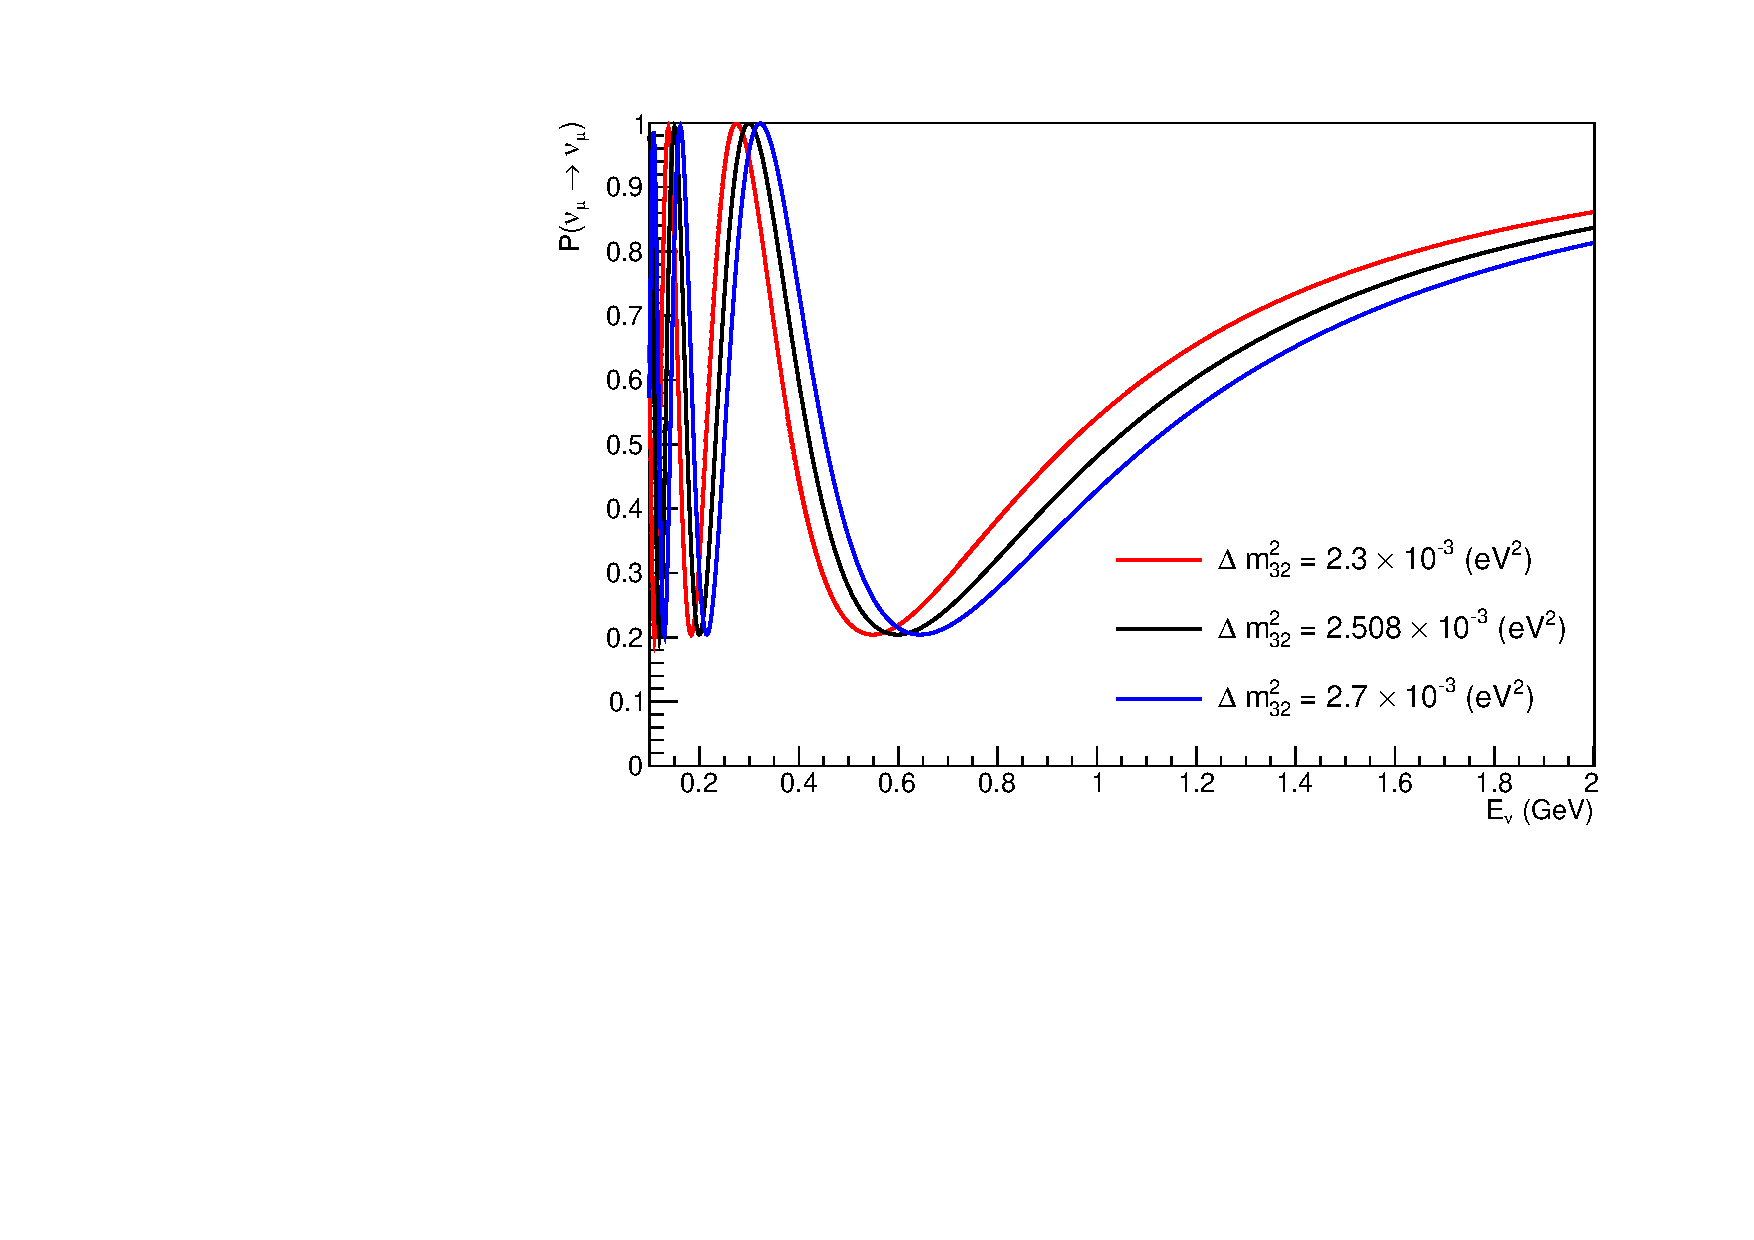
\includegraphics[width=\textwidth, trim={0mm 0mm 0mm 0mm}, clip,page=1]{Figures/Oscillation/T2K_NuMu_x_NuMu_DelMsq32Sens.pdf}
    \subcaption{\delmsqatm}
  \end{subfigure}%
  \begin{subfigure}[t]{0.5\textwidth}
    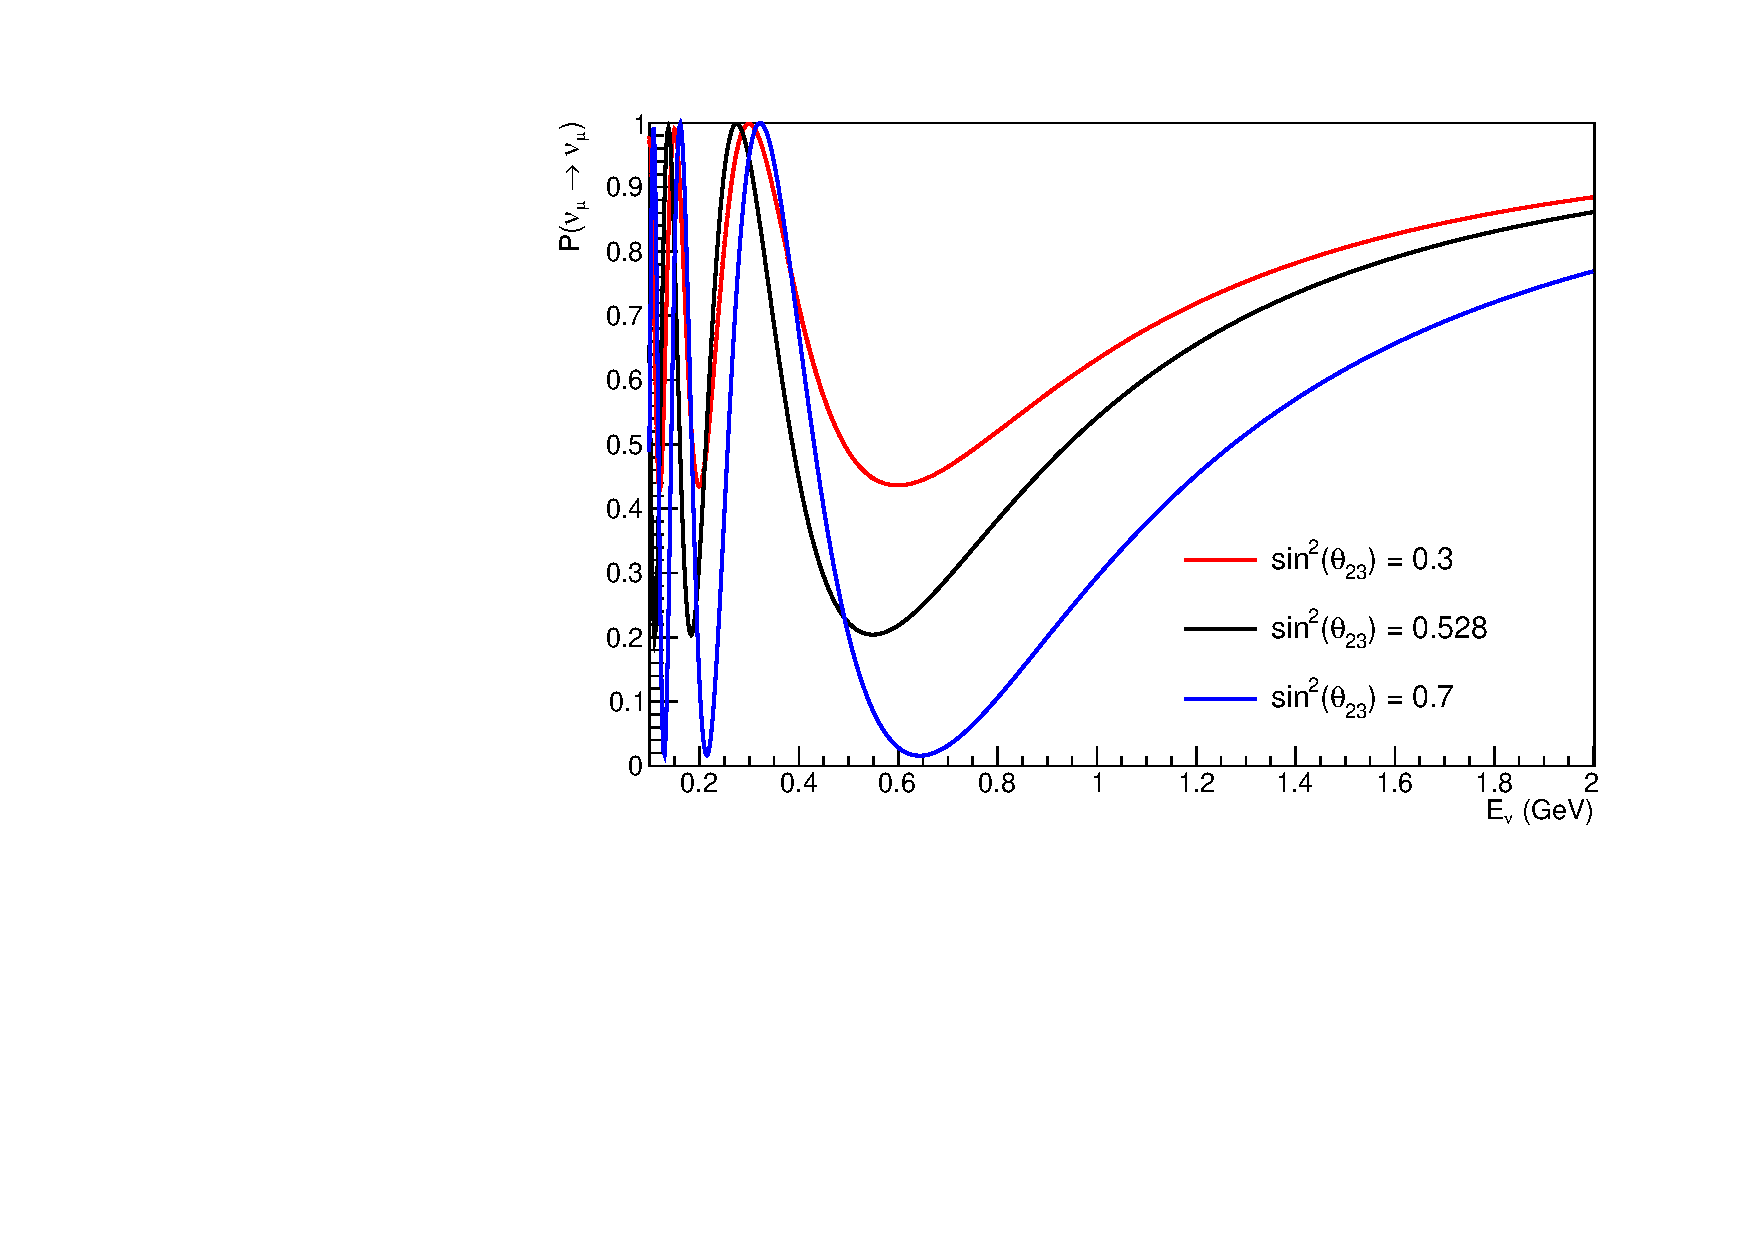
\includegraphics[width=\textwidth, trim={0mm 0mm 0mm 0mm}, clip,page=1]{Figures/Oscillation/T2K_NuMu_x_NuMu_Sinsqth23Sens.pdf}
    \subcaption{\sinsqatm}
  \end{subfigure}
  \begin{subfigure}[t]{0.5\textwidth}
    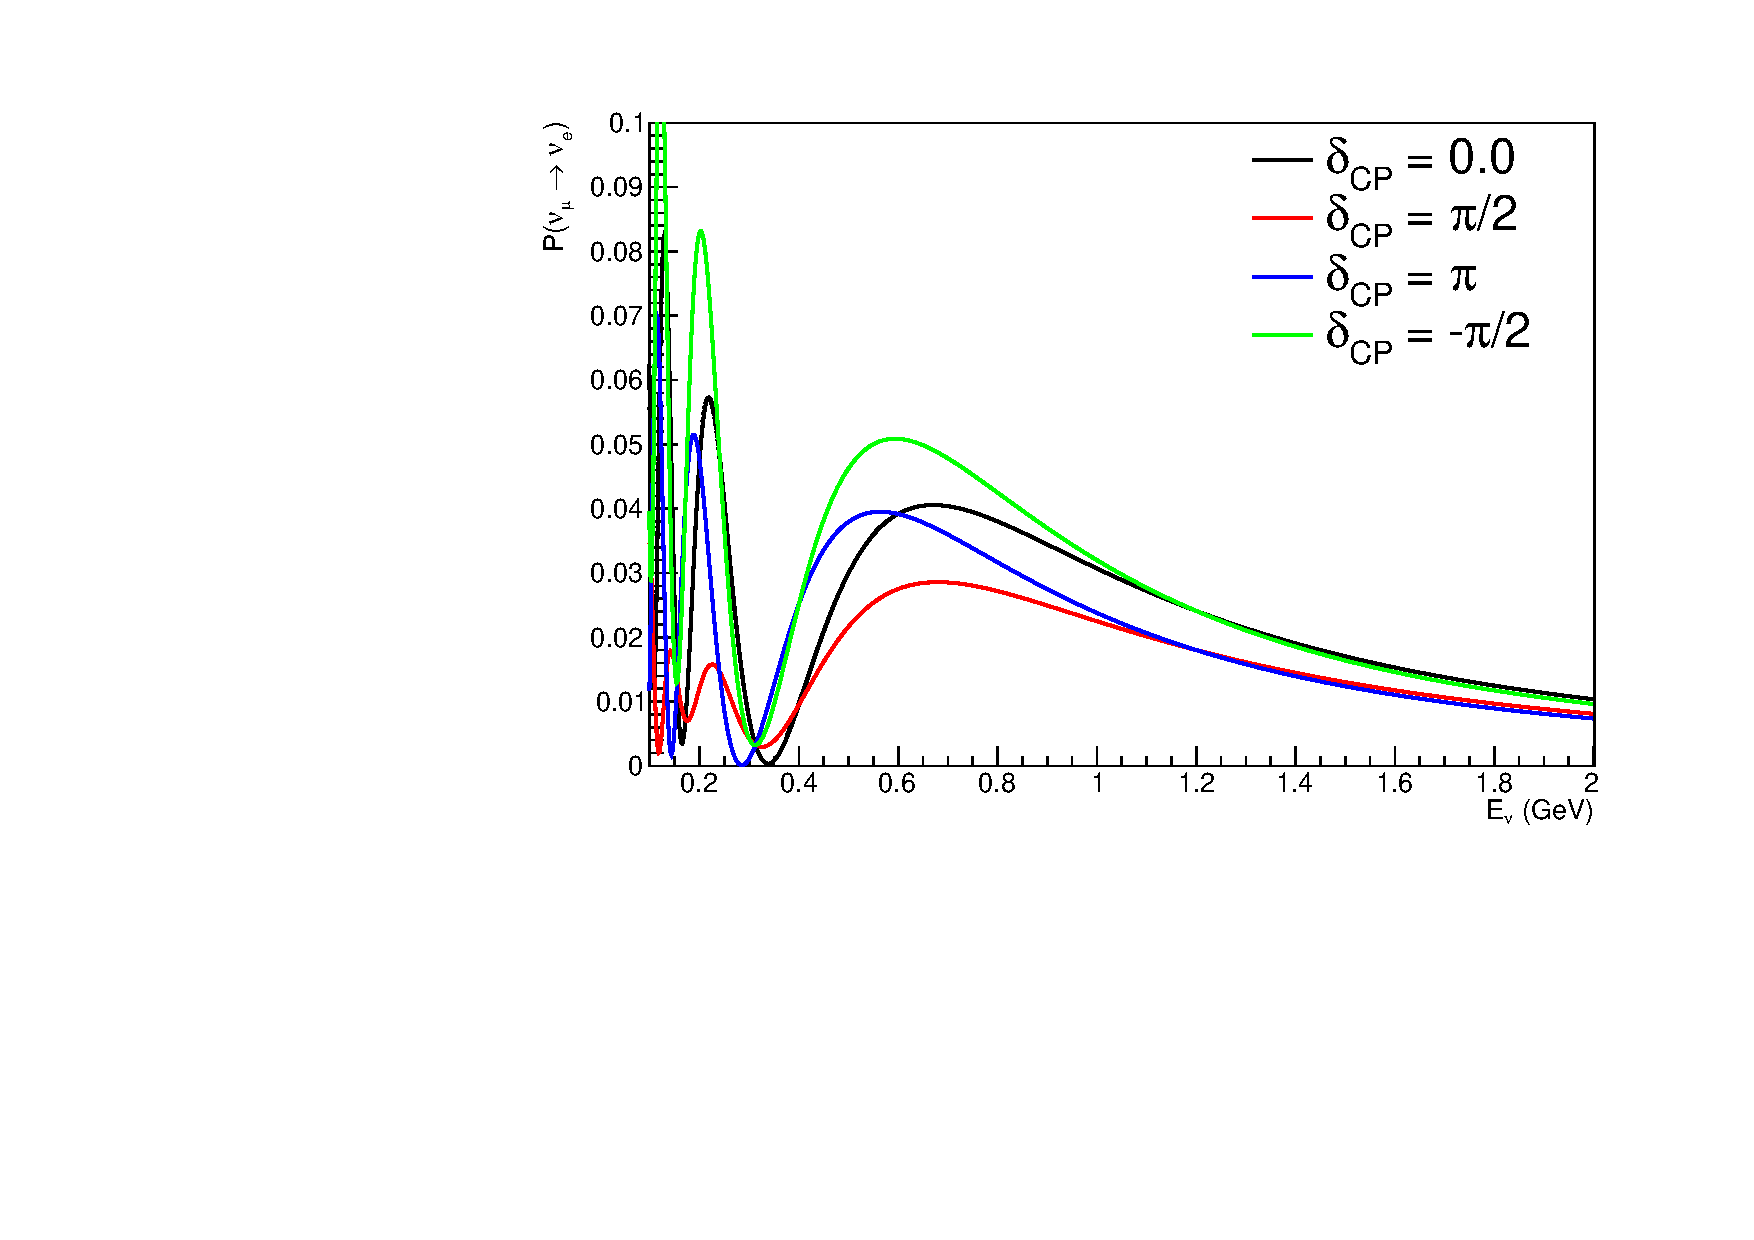
\includegraphics[width=\textwidth, trim={0mm 0mm 0mm 0mm}, clip,page=1]{Figures/Oscillation/T2K_NuMu_x_NuE_DCPSens.pdf}
    \subcaption{\dcp}
  \end{subfigure}
  \caption{The oscillation probability for beam neutrino events, given as a function of neutrino energy. All oscillation parameters assume the ``Asimov A'' set given in \autoref{tab:Oscillation_ParameterSets} unless otherwise stated. Each panel represents a change in one of the oscillation parameters whilst keeping the remaining parameters fixed.}
  \label{fig:Oscillation_T2K_OscillationProbSensitivity}
\end{figure}

T2K's sensitivity to the atmospheric oscillation parameters is more of a shape-based variation of the muon-like samples, as illustrated in \autoref{fig:Oscillation_T2K_OscillationProbSensitivity}. The value of \quickmath{\Delta m^{2}_{32}} laterally shifts the position of the oscillation dip (around \quickmath{E_\nu \sim 0.6\text{GeV}}) in the \quickmath{P(\nu_\mu \rightarrow \nu_\mu)} oscillation probability. A variation of \sinsqatm is predominantly observed as a vertical shift of the oscillation dip with second-order horizontal shifts being due to matter effects. The beam neutrinos have limited sensitivity to matter effects due to the shorter baseline as well as the Earth's mantle is relatively low-density material (as compared to the Earth's core). For some values of \dcp, the degeneracy in the number of e-like events allows the mass hierarchy to be resolved. This leads to a \dcp-dependent mass hierarchy sensitivity. \finish{Bi-probability plot?}

Whilst all oscillation channels should be included for completeness, the computational resources required to run a fit are limited and any reasonable approximations which reduce the number of oscillation probability calculations which need to be made should be applied. The \quickmath{\nu_{e} \rightarrow \nu_{e,\mu,\tau}} (and antineutrino equivalent) oscillations can be ignored for beam neutrinos as the \quickmath{\nu_{e}/\bar{\nu}_{e}} fluxes being approximately two orders of magnitude smaller than the corresponding \quickmath{\nu_{\mu}/\bar{\nu}_{\mu}} flux. Furthermore, as the peak neutrino energy of the beam is well below the threshold for \quickmath{\tau} production (\quickmath{E_\nu \sim 3\text{GeV}} \cite{Machado2020}) only a small proportion of the neutrinos produced in the beam have the required energy. For the few neutrinos that have sufficient energy, the oscillation probability is very small due to the short baseline. Whilst these approximations can be made for the beam neutrinos, the atmospheric flux of \quickmath{\nu_{e}} is of the same order of magnitude as the \quickmath{\nu_{\mu}} flux and the energy distribution of atmospheric neutrinos extends well above the tau production threshold.

Throughout this thesis, several spectra predictions, Asimov fits, and contour comparisons are presented which require oscillation parameters to be assumed. \autoref{tab:Oscillation_ParameterSets} defines two sets of oscillation parameters, with ``Asimov A'' set being close to the preferred values from a previous T2K-only fit \finish{Need Citation} and ``Asimov B'' being CP-conserving and further from maximal \quickmath{\theta_{23}} mixing.

\begin{table}[ht!]
    \centering
    \begin{tabular}{c|c|c}
      \hline
      \hline
      Parameter & Asimov A & Asimov B \\
      \hline
      \quickmath{\Delta m^{2}_{12}} & \multicolumn{2}{c}{\quickmath{7.53 \times 10^{-5} \text{eV}^{2}}} \\ \hline
      \quickmath{\Delta m^{2}_{32}} & \multicolumn{2}{c}{\quickmath{2.509 \times 10^{-3} \text{eV}^{2}}} \\ \hline
      \quickmath{\sin^{2}\left(\theta_{12}\right)} & \multicolumn{2}{c}{\quickmath{0.304}} \\ \hline
      \quickmath{\sin^{2}\left(\theta_{13}\right)} & \multicolumn{2}{c}{\quickmath{0.0219}} \\ \hline
      \quickmath{\sin^{2}\left(\theta_{23}\right)} & \quickmath{0.528} & \quickmath{0.45} \\ \hline
      \quickmath{\delta_{CP}} & \quickmath{-1.601} & \quickmath{0.0} \\ \hline
      \hline
    \end{tabular}
    \caption{Reference values of the neutrino oscillation parameters for two different oscillation parameter sets.}
    \label{tab:Oscillation_ParameterSets}
\end{table}

\section{Treatment of Fast Oscillations}
\label{sec:Oscillation_FastOscillations}

As shown in \autoref{fig:Oscillation_SK_FastOscillogram}, atmospheric neutrino oscillations have a significantly more complex structure for upgoing neutrinos with energy below \quickmath{1\text{GeV}}. This is because the \quickmath{L/E} dependence of the oscillation probability in this region induces rapid variations for small changes in \quickmath{L} or \quickmath{E}. As discussed in \autoref{sec:Oscillation_Overview}, this is also the region in which atmospheric neutrinos have sensitivity to \dcp. In practice, the direction between the detector and a neutrino's production vertex is inferred from the direction of any secondary particles created in the detector target. For low energy neutrinos, this inference can be rather poor and introduces a distinct difference to beam neutrinos where the direction to production vertex is very well known.

As a consequence of the poor detector resolution, an average oscillation probability is observed in this region. This creates a computational problem as a significantly large amount of MC statistics would be required to accurately predicted the number of events in each bin if MC averaging was the only technique used. This section describes the `sub-sampling' approach developed for this analysis and compares it to the methodology used within the SK-only analysis.

\begin{figure}[h]
  \begin{subfigure}[t]{0.8\textwidth}
    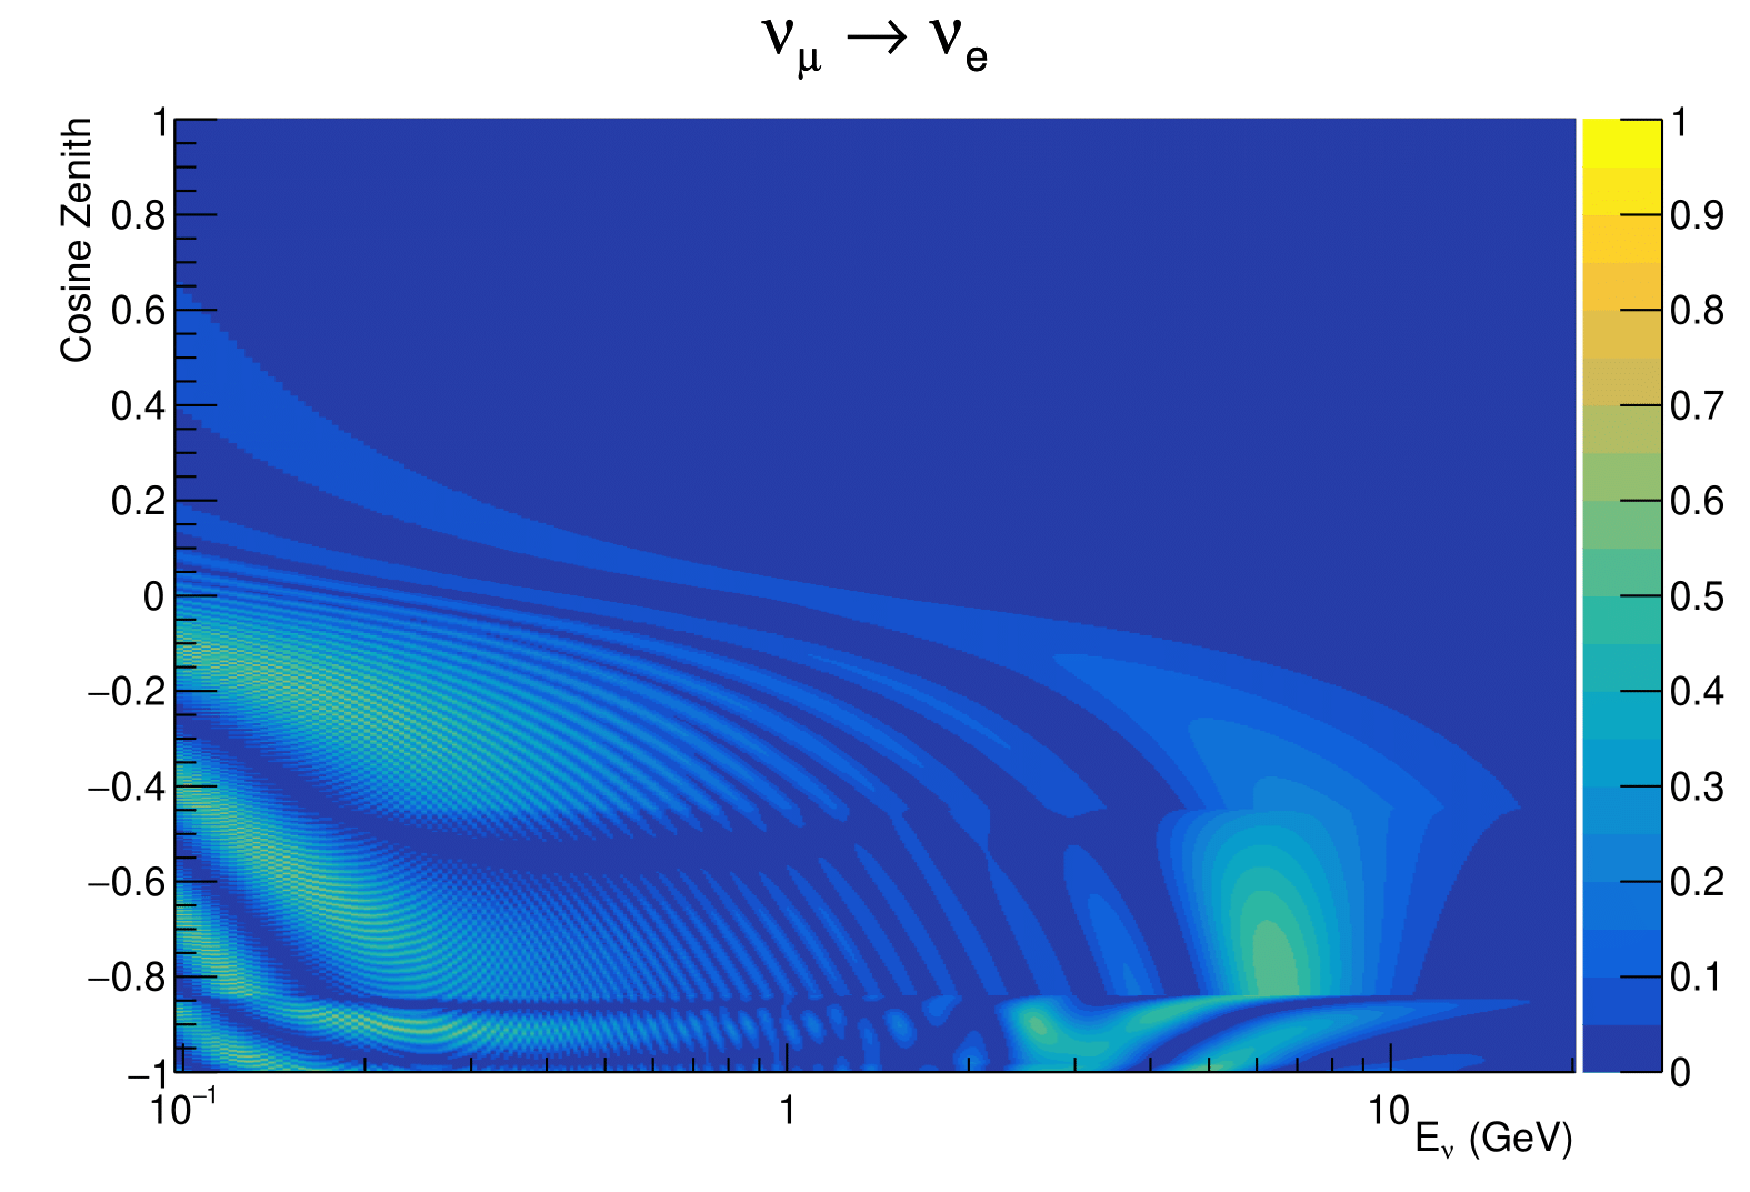
\includegraphics[width=\textwidth, trim={0mm 0mm 0mm 0mm}, clip,page=1]{Figures/Oscillation/FastOscillationExample.pdf}
  \end{subfigure}
  \caption{The oscillation probability \quickmath{P(\nu_{\mu} \rightarrow \nu_{e})}, given as a function of neutrino energy and zenith angle, which highlights an example of the ``fast'' oscillations in the sub-GeV upgoing region.}
  \label{fig:Oscillation_SK_FastOscillogram}
\end{figure}

The official SK-only analysis uses the osc3++ oscillation parameter fitter \cite{thesis_roger}. To perform the fast oscillation averaging, it uses a 'nearest-neighbour' technique. For a given neutrino MC event, the nearest neighbours in reconstructed lepton momentum and zenith angle are found and a distribution of neutrino energies is built. This distribution is then used to compute an average oscillation probability for the given neutrino MC event. 

For the \quickmath{i^{th}} event, the oscillation weight is calculated as

\begin{equation}
  W_{i} = \frac{1}{5} P(E_{i},\bar{L}_{i}) + \frac{1}{5} \sum_{\beta = -1, -0.5, 0.5, 1} P(E_{i} + \beta\sigma_{i},L_{\beta}),
\end{equation}

where \quickmath{P(E,L)} is the oscillation probability calculation for neutrino energy \quickmath{E} and path length \quickmath{L}, \quickmath{\sigma_{i}} is the RMS of the energy distribution for the given event, and the two path lengths, \quickmath{\bar{L}_{i}} and \quickmath{L_{\beta}} are discussed below. In practice, twenty of the nearest neighbours are used to generate the neutrino energy distribution. All of the oscillation probability calculations are performed with a fixed zenith angle (and therefore have same matter density profile).

The uncertainty in the production height is controlled by using an ``average'' production height. \quickmath{\bar{L}_{i}} represents the average path length computed using twenty production heights taken from the Honda flux model's prediction \finish{Need citation} for a fixed zenith angle, where the production heights are sampled in steps of \quickmath{5\%} of their cumulative distribution function. \quickmath{L_{\beta}} values are similarly calculated but instead use different combinations of four production heights (sampled in the same way),

\begin{equation}
  \begin{split}
    L_{-1.0} &= \frac{1}{4} L(45,50,55,60), \\
    L_{-0.5} &= \frac{1}{4} L(35,40,65,70), \\
    L_{+0.5} &= \frac{1}{4} L(25,30,75,68), \\
    L_{+1.0} &= \frac{1}{4} L(15,20,85,89). \\
  \end{split}
\end{equation}

This averaging works well because of the correlation between true neutrino zenith angle and the inferred direction from secondary particles in the detector. For low energy neutrinos, where the resolution of the true neutrino direction is poor, \quickmath{\sigma_{i}} will be large resulting in significant averaging effects. Contrary to this, the inferred direction of high energy neutrinos will be much closer to the true value, meaning that \quickmath{\sigma_{i}} will be smaller.

In practice, this technique is performed before the fit in order to deal with the computational cost. Oscillation probabilities are pre-calculated on a 4D grid. This is possible as the Osc3++ framework uses binned oscillation parameters rather than continous so the oscillation parameters used in the fit are known prior to run-time. The framework used in the analysis presented within this thesis uses continous oscillation parameters. Due to the MCMC technique invoked within the fitter (\finish{Link to MCMC chapter}), there is no way to know which oscillation parameter values will be selected in each step at run-time. Therefore, the oscillation parameter calculation would have to be performed at run-time which is very expensive for event-by-event reweighting. Having to compute five oscillation probabilities per event would require far too much computational resources to be viable so the SK technique can not be used within this analysis. However, the concept of the averaging technique can be taken from it.

\begin{figure}[h]
  \begin{subfigure}[t]{\textwidth}
    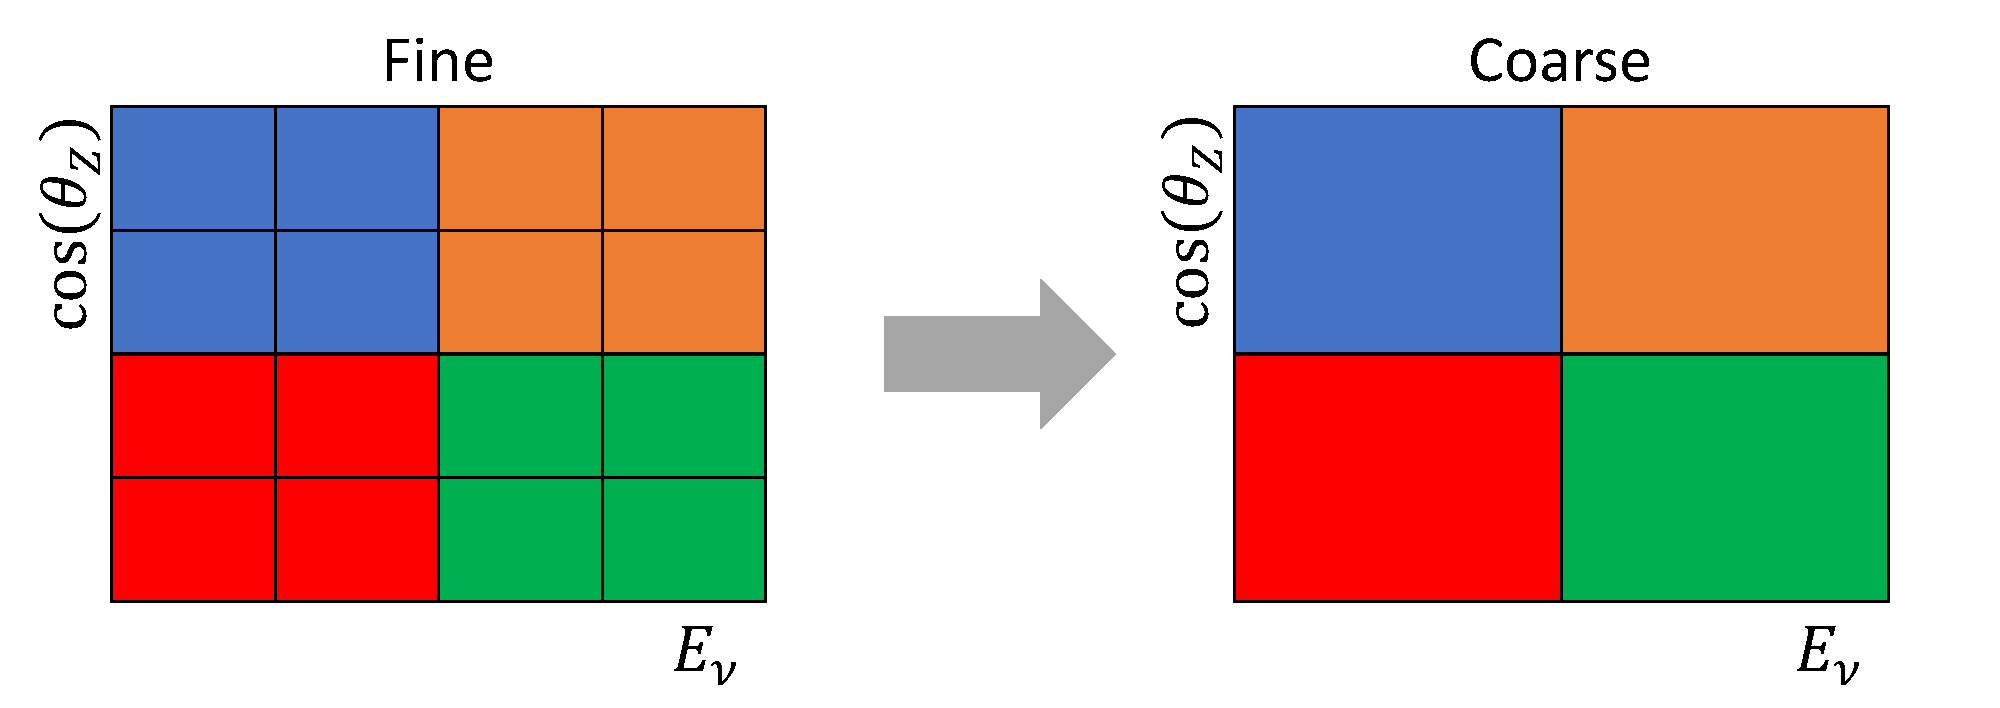
\includegraphics[width=\textwidth, trim={0mm 0mm 0mm 0mm}, clip,page=1]{Figures/Oscillation/SubSamplingExample.pdf}
  \end{subfigure}
  \caption{Illustration of the averaging procedure for \quickmath{N=2}. The oscillation probabilities calculated on the finer left binning are averaged to obtain the oscillation probabilities in the coarser right binning. These averaged oscillation probabilities with the coarser binning are then applied to each event during the fit.}
  \label{fig:Oscillation_SK_SubSamplingExample}
\end{figure}

This analysis uses a binned oscillogram in which oscillation probabilities for a given event are selected based on that event's attributes. To perform a similar averaging as the SK analysis, a sub-sampling approach has been devised. The technique can be explained by considering a ``fine'' and ``coarse'' oscillogram. The fine oscillograms are used to define the array of cosine zeniths and energies for the neutrino oscillation engine. The coarse oscillograms cover the same phasespace as the fine oscillograms but have fewer bins in that range. Then, for a given coarse oscillogram bin, the value of that bin will be taken as the average of all the oscillation probabilities of all the fine oscillogram bins which fall into that coarse oscillogram bin.

The binning which is used to calculate the oscillation probabilities, known as the `fine' binning, has \quickmath{N \times N} subdivisions per coarse bin. The value assigned to a coarse bin is the linear average (flat prior in \quickmath{E_{\nu}} and \quickmath{\cos(\theta_{Z})}) of all the oscillation probabilities calculated at the center of each fine bin contained within that coarse bin. \autoref{fig:Oscillation_SK_SubSamplingExample} illustrates the \quickmath{N = 2} example where the assigned value to a coarse bin is the linear average of the four fine bins which fall in that coarse bin. Whilst the coarse bin edges are not linear in either axis, the sub-division of the fine bins is linear over the range of a coarse bin. The alignment of the fine and coarse binning edges are checked at run-time.

The coarse binning is defined with \quickmath{67 \times 52} bins in true neutrino energy \quickmath{\times} cosine zenith. In general, the binning is logarithmically spaced in neutrino energy but has some hand-picked bin edges. Firstly, the bin density around the matter resonance is smoothly increased around the matter resonance region. This is to avoid smearing this region which can be well sampled by the Monte Carlo. Secondly, bin edges are selected to hit \quickmath{0.4, 0.6, 1, 10, 30, 50, 100 \text{GeV}}. This is to ensure that the Coloumb correction systematic and the atmospheric flux systematics definitions in neutrino energy can be hit. The cosine zenith binning is approximately linearly spaced across the allowable range but the values of layer transitions are hit precisely; \quickmath{-0.8376} (core-mantle) and \quickmath{-0.4464} (mantle/transition zone). Bins are spread further apart for downgoing events as this is a region unaffected by the fast oscillation wavelengths and reduces the total number of calculations required to perform the reweight (Not the number required to perform the oscillation calculation).

The choice of \quickmath{N} is justified based on two studies. Firstly, the variation of event rates of each sample is studied as a function of the number of subdivisions. For a given set of oscillation parameters thrown from the PDG prior constraints, the oscillation probabilities are calculated using a given value of \quickmath{N}. Each sample is re-weighted and the event rate is stored. The value of \quickmath{N} is scanned from \quickmath{1}, which corresponds to no averaging, to \quickmath{24}, which corresponds to the largest computationally viable subdivision binning. The event rate of each sample at large \quickmath{N} is expected to converge to a stationary value due to the fine binning fully sampling the small scale structure. \autoref{fig:Oscillation_SK_EventRateVariable} illustrates this behaviour for the \texttt{SubGeV\_elike\_0dcy} sample for \quickmath{30} different throws of the oscillation parameters.

\begin{figure}[h]
  \begin{subfigure}[t]{\textwidth}
    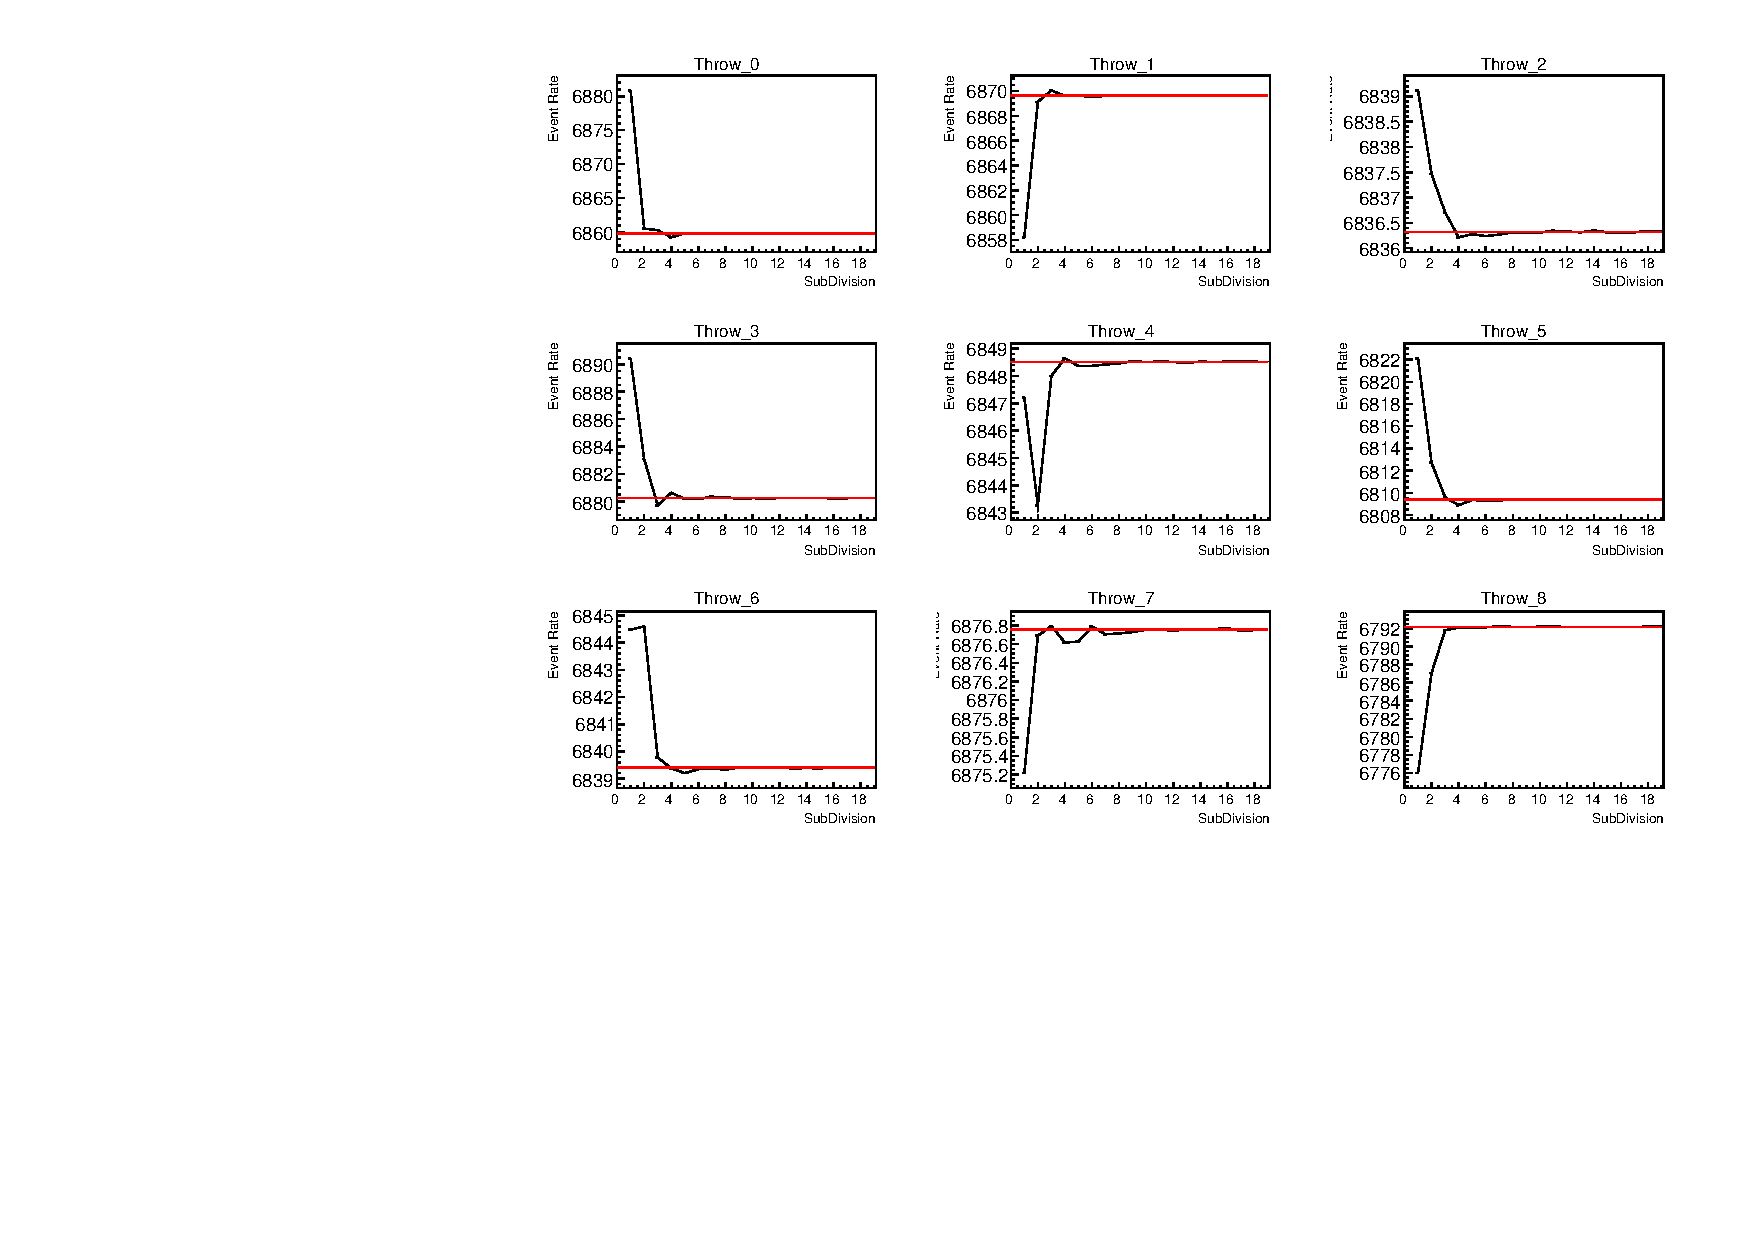
\includegraphics[width=\textwidth, trim={0mm 0mm 0mm 0mm}, clip,page=1]{Figures/Oscillation/EventRate_VariableGraphs.pdf}
  \end{subfigure}
  \caption{Event rate of the \texttt{SubGeV\_elike\_0dcy} sample as a function of the number of sub-divisions per coarse bin. Each sub-plot represents the event rate of the sample at a different oscillation parameter set (thrown from the PDG priors). The red-line in each sub plot represents the mean of the event rate over the different values of sub divisions for that particular oscillation parameter throw.}
  \label{fig:Oscillation_SK_EventRateVariable}
\end{figure}

Denoting the event rate for one sample for a given throw \quickmath{t} at each \quickmath{N} by \quickmath{\lambda_t^{(N)}}, the average over all considered \quickmath{N} values (\quickmath{\overline \lambda_t = \frac{1}{24} \sum_{N=1}^{24} \lambda_t^{(N)}}) is computed. The variance in the event rate at each \quickmath{N} is then calculated from

\begin{equation}
  \mathrm{Var}\Big[\lambda^{(N)} - \overline \lambda\Big] = \tfrac{1}{N_\mathrm{throws}} \sum_{t=1}^{N_\mathrm{throws}} \left(\lambda_t^{(N)} - \overline \lambda_t\right)^2 - \left[\tfrac{1}{N_\mathrm{throws}} \sum_{t=1}^{N_\mathrm{throws}} \left(\lambda_t^{(N)} - \overline \lambda_t\right)\right]^2 .
  \label{eq:Oscillation_SK_Variance}
\end{equation}

The aim of the study is to find the lowest value of \quickmath{N} such that this variance is below \quickmath{0.001}. This is the typical threshold used by T2K fitters to validate systematic implementation so is just as applicable to the oscillation probability calculation. The results of this study for each atmospheric sample used within this thesis are illustrated in \autoref{fig:Oscillation_SK_EventRateVariance} for \quickmath{2000} throws of the oscillation parameters. As can be seen, the variance is below the threshold at \quickmath{N = 10}, and is driven primarily by the \texttt{SubGeV\_mulike\_1dcy} and \text{SubGeV\_elike\_0dcy} selections.

\begin{figure}[h]
  \begin{subfigure}[t]{\textwidth}
    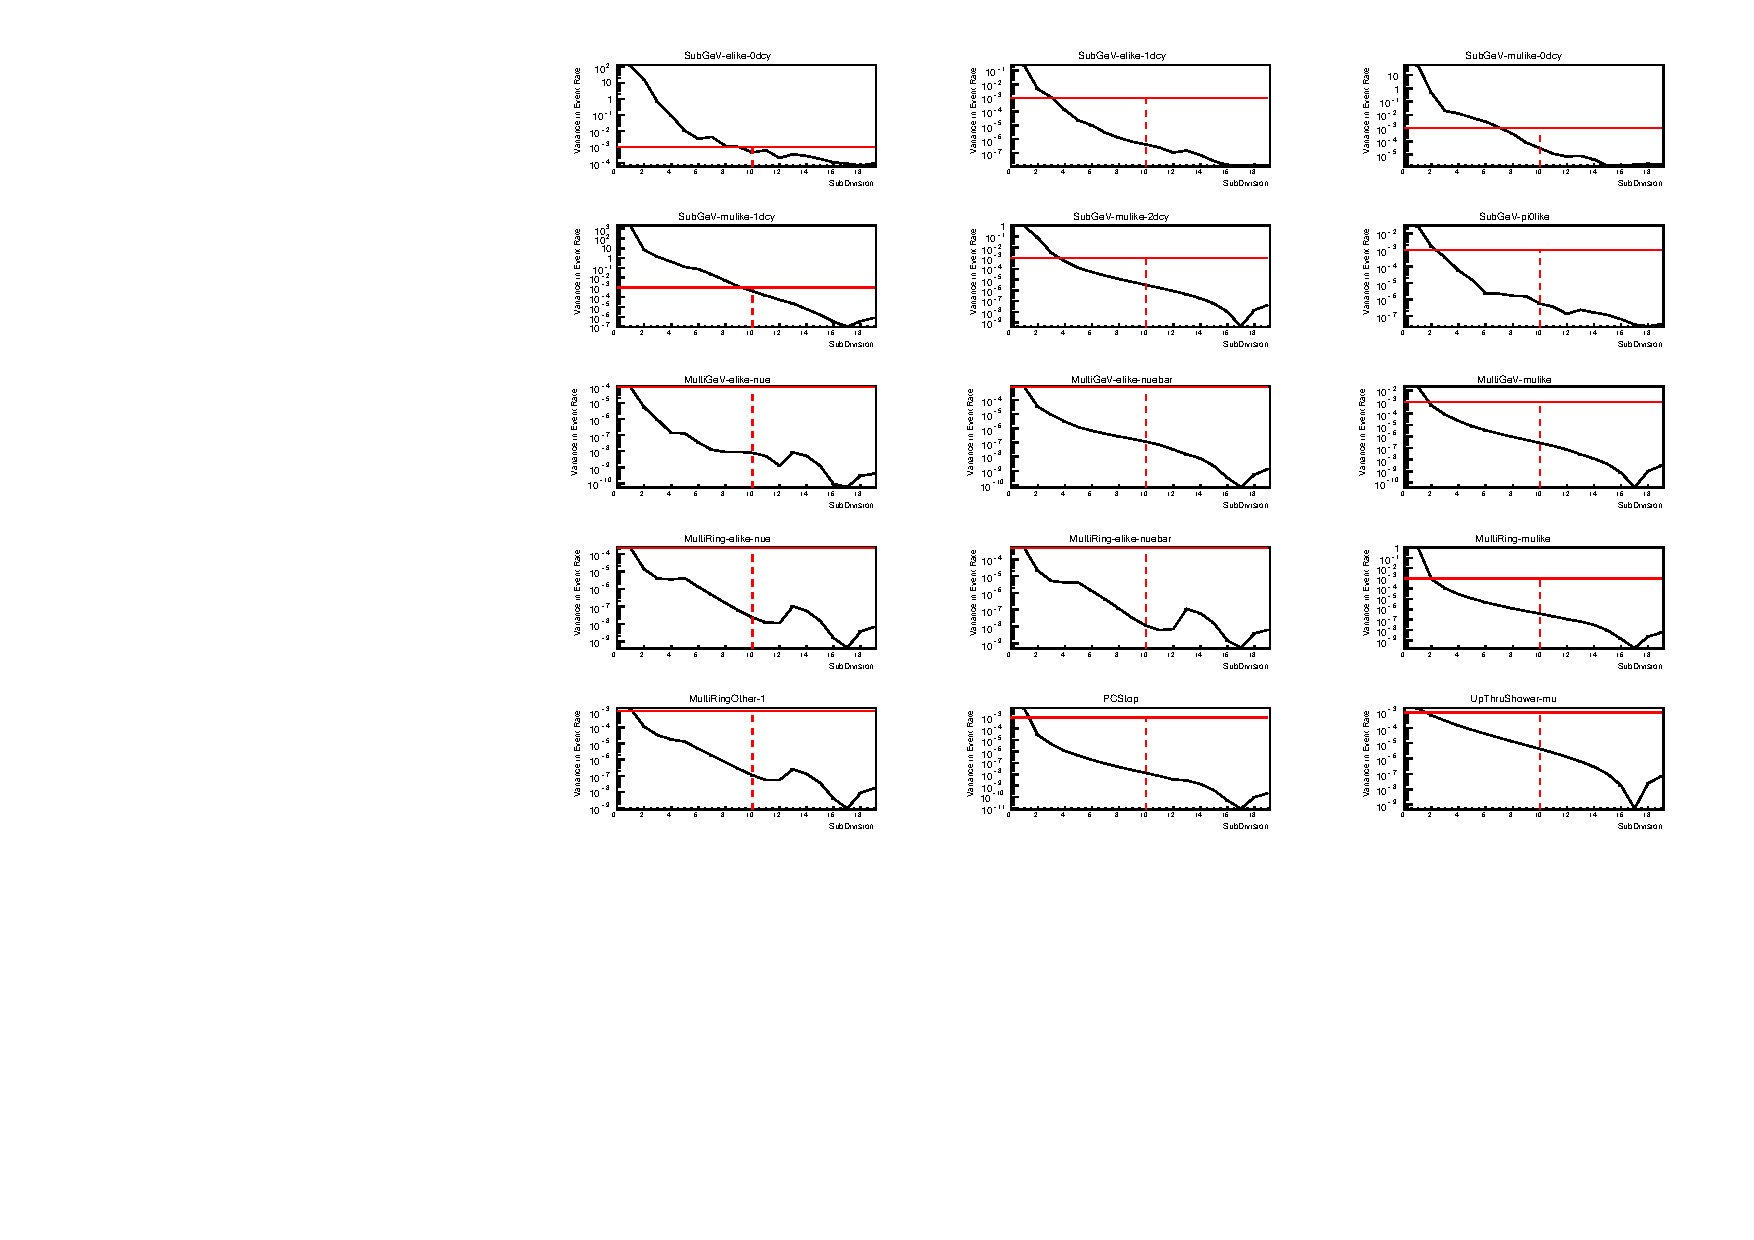
\includegraphics[width=\textwidth, trim={0mm 0mm 0mm 0mm}, clip,page=1]{Figures/Oscillation/EventRate_VarianceGraphs.pdf}
  \end{subfigure}
  \caption{Variance of event rate for each atmospheric sample as a function of the number of sub-divisions per coarse bin. The solid red line indicates the \quickmath{0.1\%} threshold and the dashed red line is a graphical indication of the variance at a sub-division \quickmath{N = 10}.}
  \label{fig:Oscillation_SK_EventRateVariance}
\end{figure}

The second study to determine the value of \quickmath{N} is as follows. The likelihood for each sample is computed against an Asimov data set created with oscillation parameters from ``Asimov A'' in \autoref{tab:Oscillation_ParameterSets}. Following \autoref{eq:Oscillation_SK_Variance}, the variance of the log-likelihood over all considered \quickmath{N} is computed. The results are shown in \autoref{fig:Oscillation_SK_LLHVariance}. This tests the impact of the averaging on each sample's binning by reconstructed momentum and/or zenith angle and also provides a scale for the calculation errors compared to their statistical uncertainties. 

\begin{figure}[h]
  \begin{subfigure}[t]{\textwidth}
    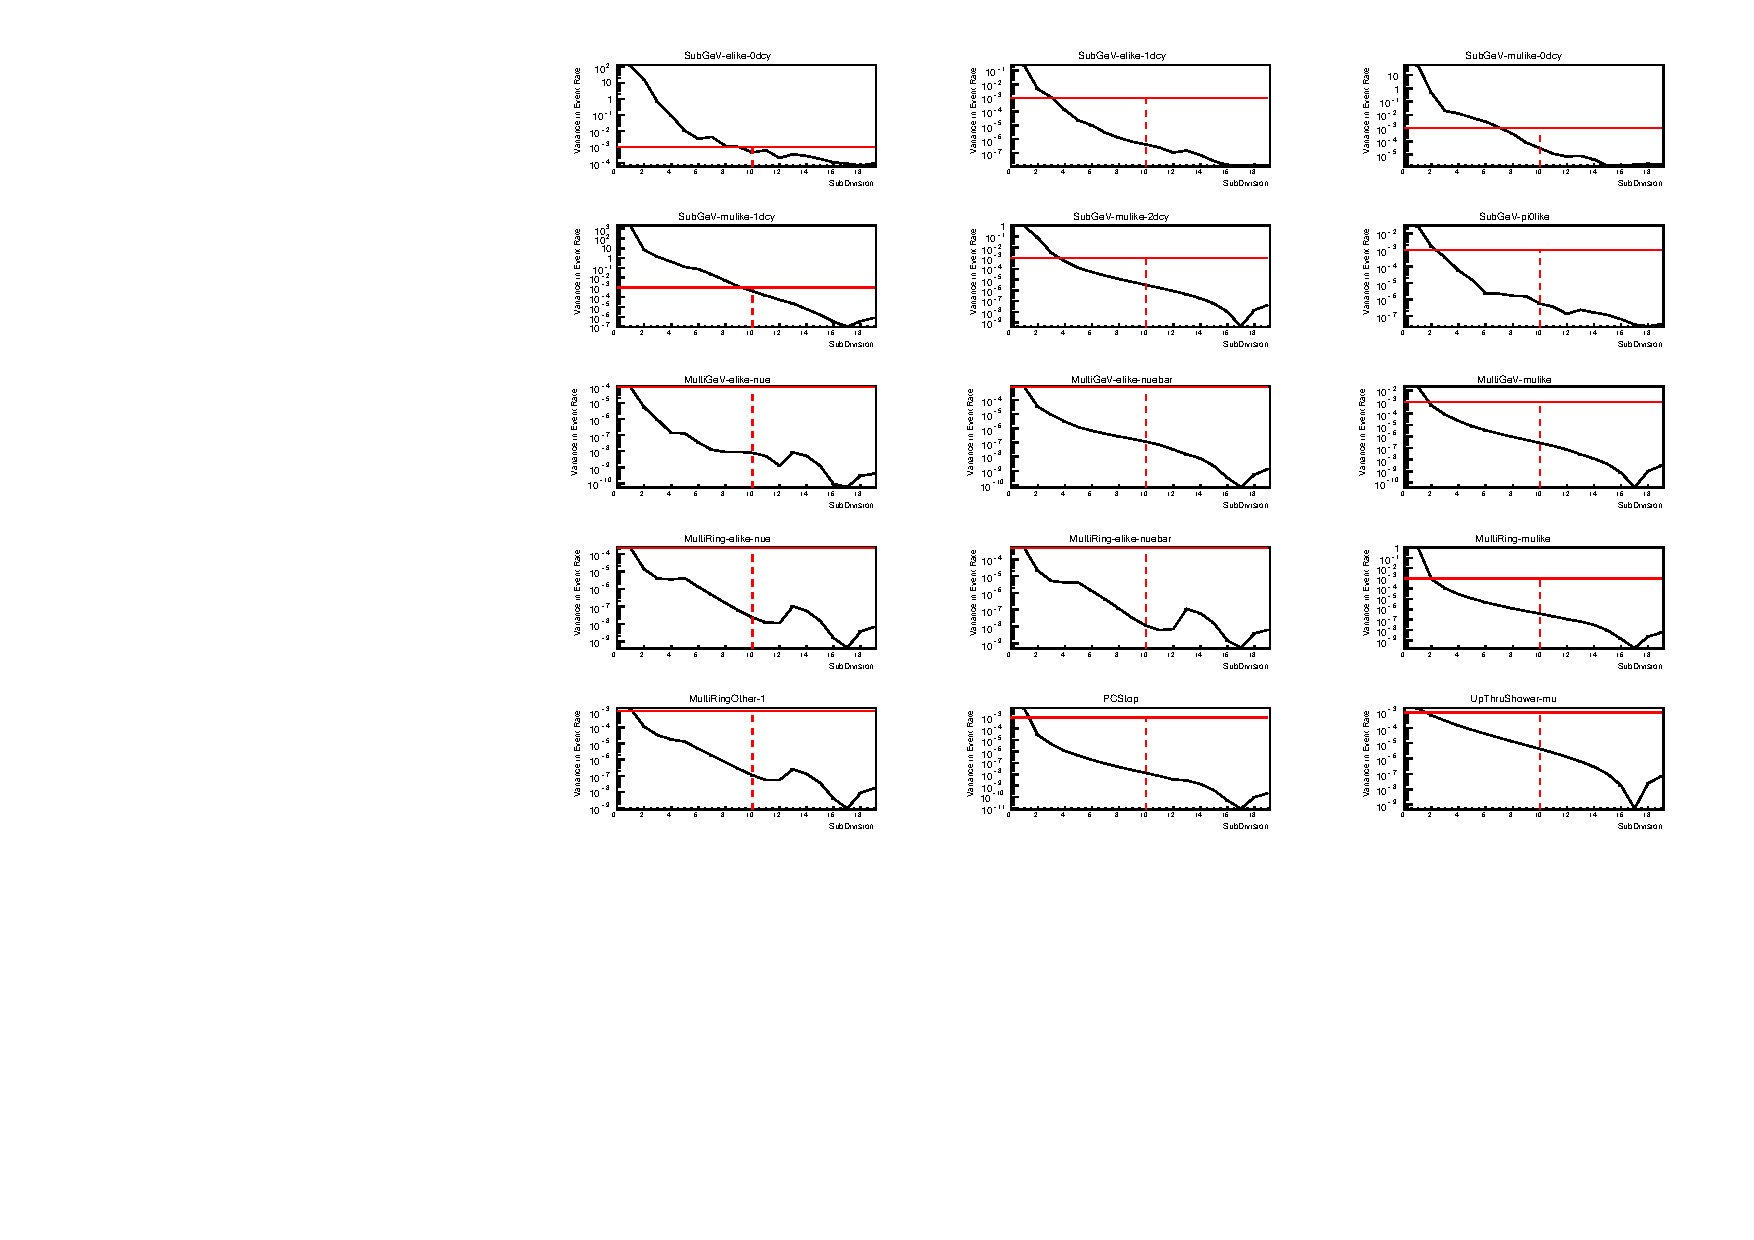
\includegraphics[width=\textwidth, trim={0mm 0mm 0mm 0mm}, clip,page=1]{Figures/Oscillation/EventRate_VarianceGraphs.pdf}
  \end{subfigure}
  \caption{Variance of sample likelihood, when compared to `Asimov data' set at Asimov A, for each atmospheric sample as a function of the number of sub-divisions per coarse bin. The solid red line indicates the \quickmath{0.1\%} threshold and the dashed red line is a graphical indication of the variance at a sub-division \quickmath{N = 10}.}
  \label{fig:Oscillation_SK_LLHVariance}
\end{figure}

A choice of \quickmath{N} sub-divisions per coarse bin has a variance in both event rate and log-likelihood residuals less than the required threshold of \quickmath{0.001}. The event rate test is the more stringent test. For the variance of log-likelihood residuals the largest value is of order \quickmath{10^{-7}}, corresponding to an error on the log-likelihood of about \quickmath{3\times 10^{-4}}, small enough to be negligible for the oscillation analysis.
